\documentclass[a4paper]{article} 
\usepackage{graphicx} 
\usepackage[ngerman]{babel} 
\usepackage[ansinew]{inputenc} 
\usepackage[T1]{fontenc} 
\usepackage{tgpagella} 
\usepackage{geometry} 
\usepackage{color} 
\usepackage{microtype} 
\usepackage{minted}
\usepackage{caption}
\usepackage[headsepline,footsepline]{scrpage2}
\usepackage{textcomp}
\usepackage{pdfpages}
\usepackage{mdframed}



\makeatletter
\renewcommand\minted@pygmentize[2][\jobname.pyg]{
  \def\minted@cmd{pygmentize -l #2 -f latex -F tokenmerge
    \minted@opt{gobble} \minted@opt{texcl} \minted@opt{mathescape}
    \minted@opt{startinline} \minted@opt{funcnamehighlighting}
    \minted@opt{linenos} -P "verboptions=\minted@opt{extra}"
    -O encoding=UTF-8,outencoding=iso-8859-1 -o \jobname.out.pyg #1}
  \immediate\write18{\minted@cmd}
  % For debugging, uncomment:
  %\immediate\typeout{\minted@cmd}
  \ifthenelse{\equal{\minted@opt@bgcolor}{}}
   {}
   {\begin{minted@colorbg}{\minted@opt@bgcolor}}
  \input{\jobname.out.pyg}
  \ifthenelse{\equal{\minted@opt@bgcolor}{}}
   {}
   {\end{minted@colorbg}}
  \DeleteFile{\jobname.out.pyg}}
\makeatother


\title{Dokumentation - 6 Übung}
\author{Roman Lumetsberger}
\date{\today}

\newmintedfile[ccode]{cpp}{
               linenos,
               numbersep=5pt,
               frame=lines,
               framesep=2mm
}

\newmintedfile[javacode]{java}{
               linenos,
               numbersep=5pt,
               frame=lines,
               tabsize=2,
               framesep=2mm,
}
\newmintedfile[csscode]{css}{
               linenos,
               numbersep=5pt,
               frame=lines,
               tabsize=2,
               framesep=2mm,
}
\newmintedfile[sqlcode]{sql}{
               linenos,
               numbersep=5pt,
               frame=lines,
               tabsize=2,
               framesep=2mm,
}
\captionsetup{
  font=footnotesize,
  justification=raggedright,
  singlelinecheck=false
}


\newcommand{\srcDir}{../Beispiel/src/at/lumetsnet/caas/}
\newcommand{\testDir}{../Beispiel/test/at/lumetsnet/caas/test/}

\definecolor{lineColor}{RGB}{151,0,0}
\pagestyle{scrheadings}
\clearscrheadfoot
\begin{document}
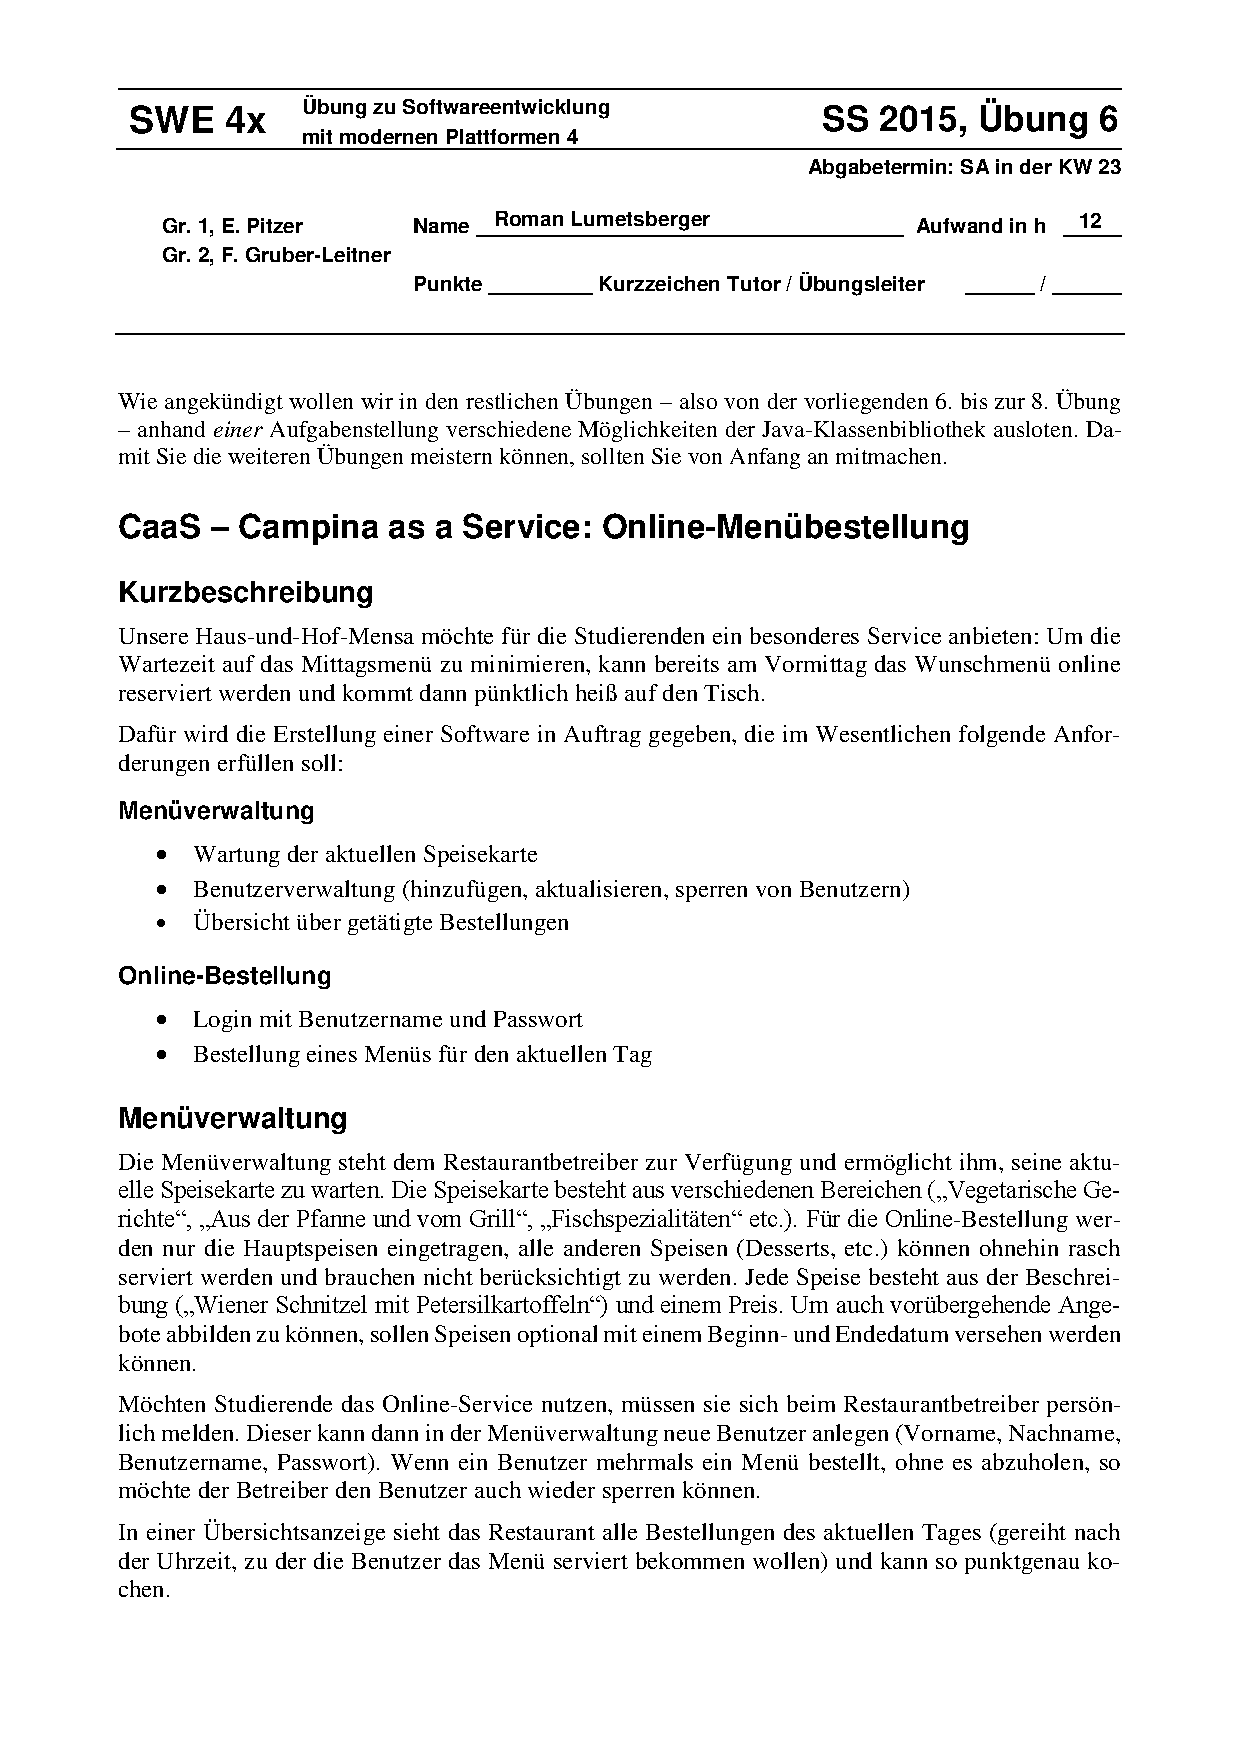
\includepdf[pages=-]{angabe.pdf}

\ihead{SWO3 SS 2015 - �bung 06}
\ifoot{Roman Lumetsberger}
\cfoot{1310307026}
\ofoot{Seite \pagemark}

\section{CaaS � Campina as a Service}
\subsection{L�sungsidee}
Da es bei dieser Aufgabe um einen GUI Prototypen geht ist es besonders wichtig, die Business-Logik nicht mit der GUI zu vermischen. \newline
Ein Ansatz das zu erreichen ist es, die Business-Logik in eigene Klassen auszulagern. \newline Diese k�nnen dann als Singleton verwendet werden.\newline
Weiters sollte die Gui mit eigenen Datenobjekten arbeiten um nicht von der Struktur der Datenhaltung abh�ngig zu sein.

\pagebreak
\includepdf[pages=-]{mockup.pdf}

\pagebreak
\subsection{Sourcecode}
\javacode{\srcDir/Main.java}
\javacode{\srcDir/business/MenuService.java}
\javacode{\srcDir/business/OrderService.java}
\javacode{\srcDir/business/UserService.java}
\javacode{\srcDir/business/Util.java}
\javacode{\srcDir/gui/ActionTableCell.java}
\javacode{\srcDir/gui/AmountTableCell.java}
\javacode{\srcDir/gui/DateTableCell.java}
\javacode{\srcDir/gui/MainWindow.java}
\javacode{\srcDir/gui/ManageUserActionCell.java}
\javacode{\srcDir/gui/Util.java}
\javacode{\srcDir/gui/dialogs/Dialog.java}
\javacode{\srcDir/gui/dialogs/ErrorDialog.java}
\javacode{\srcDir/gui/dialogs/ManageEntityDialog.java}
\javacode{\srcDir/gui/dialogs/ManageMenuCategoryDialog.java}
\javacode{\srcDir/gui/dialogs/ManageMenuDialog.java}
\javacode{\srcDir/gui/dialogs/ManageUserDialog.java}
\javacode{\srcDir/gui/pages/ManageMenusPage.java}
\javacode{\srcDir/gui/pages/ManageUsersPage.java}
\javacode{\srcDir/gui/pages/OrdersPage.java}
\javacode{\srcDir/gui/pages/Showable.java}
\javacode{\srcDir/model/Entity.java}
\javacode{\srcDir/model/Menu.java}
\javacode{\srcDir/model/MenuCategory.java}
\javacode{\srcDir/model/Order.java}
\javacode{\srcDir/model/User.java}
\javacode{\srcDir/viewmodel/ManageMenusViewModel.java}
\javacode{\srcDir/viewmodel/ManageUsersViewModel.java}
\javacode{\srcDir/viewmodel/MenuCategoryViewModel.java}
\javacode{\srcDir/viewmodel/MenuViewModel.java}
\javacode{\srcDir/viewmodel/OrdersPageViewModel.java}
\javacode{\srcDir/viewmodel/OrderViewModel.java}
\javacode{\srcDir/viewmodel/UserViewModel.java}


\pagebreak
\subsection{Testf�lle}
\begin{mdframed}
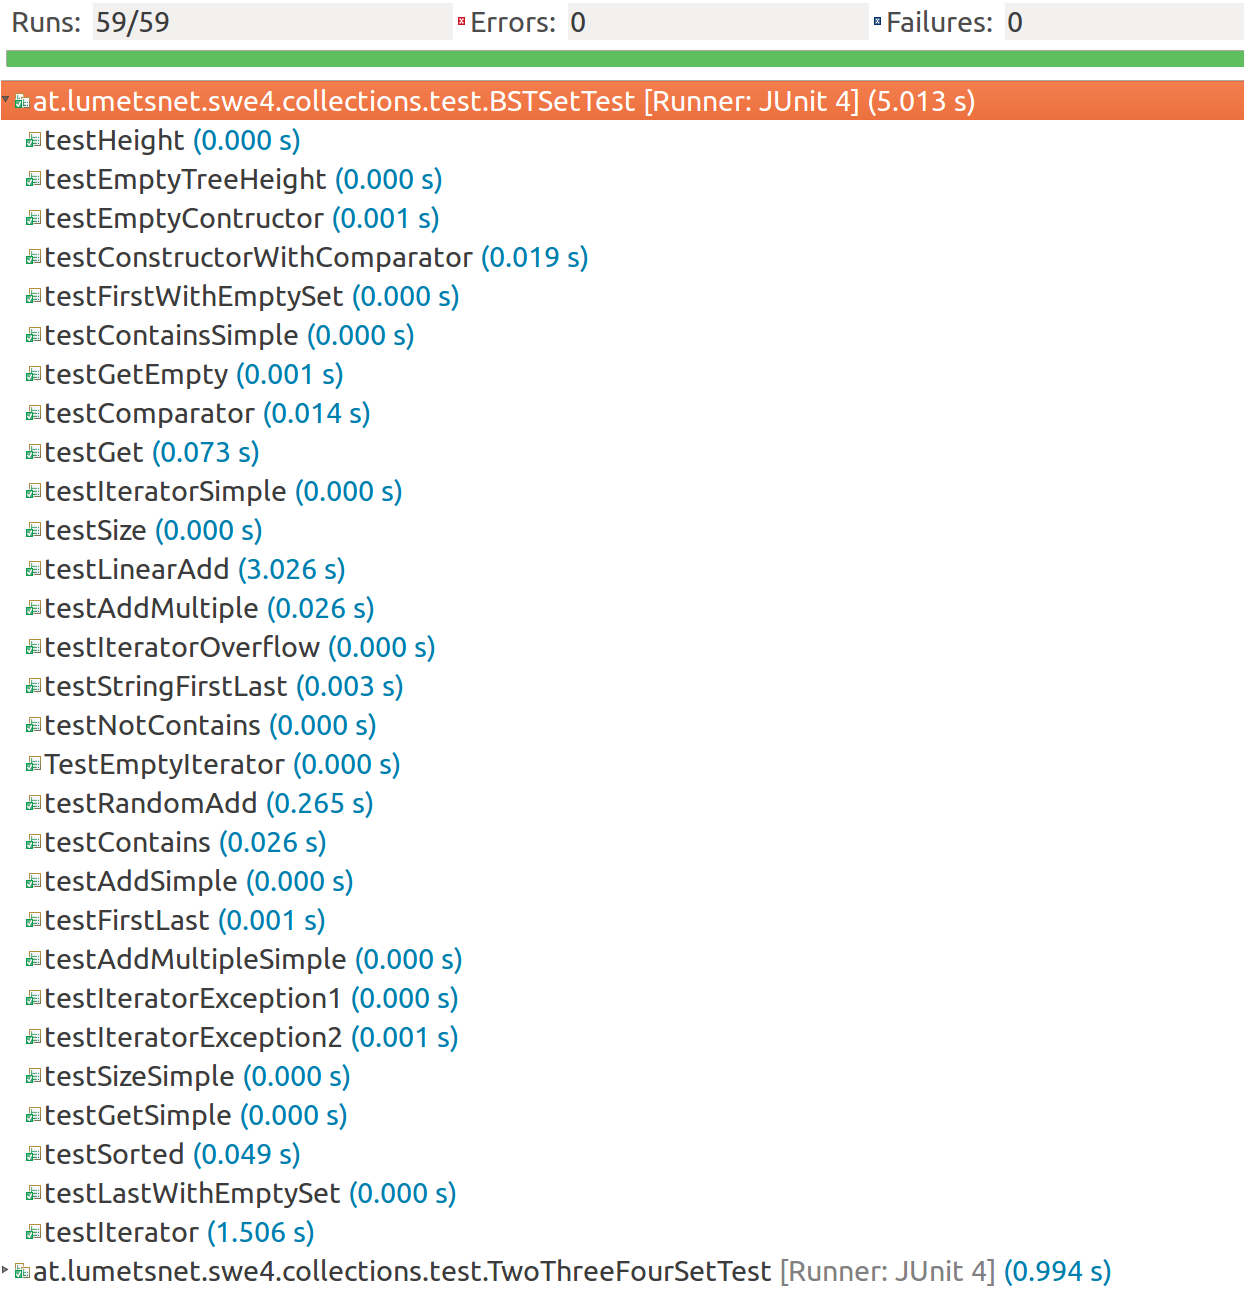
\includegraphics[width=300px]{../Screenshots/1.png}
\end{mdframed}
\begin{mdframed}
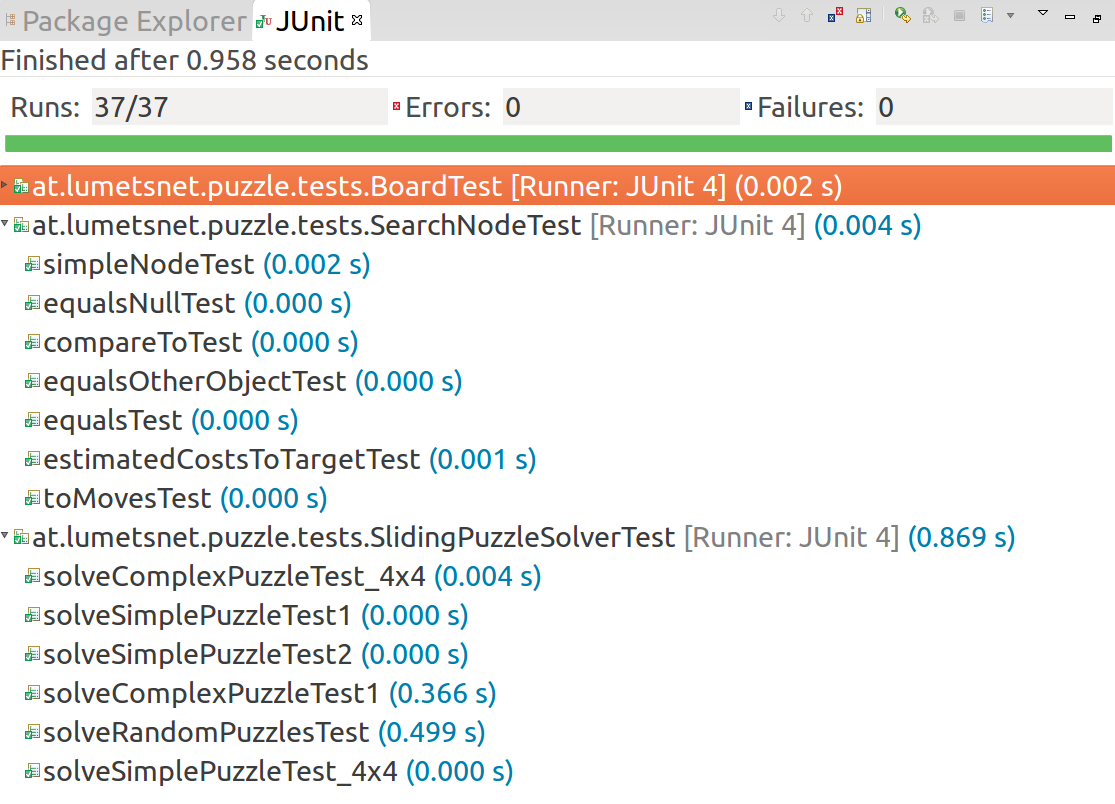
\includegraphics[width=300px]{../Screenshots/2.png}
\end{mdframed}
\begin{mdframed}
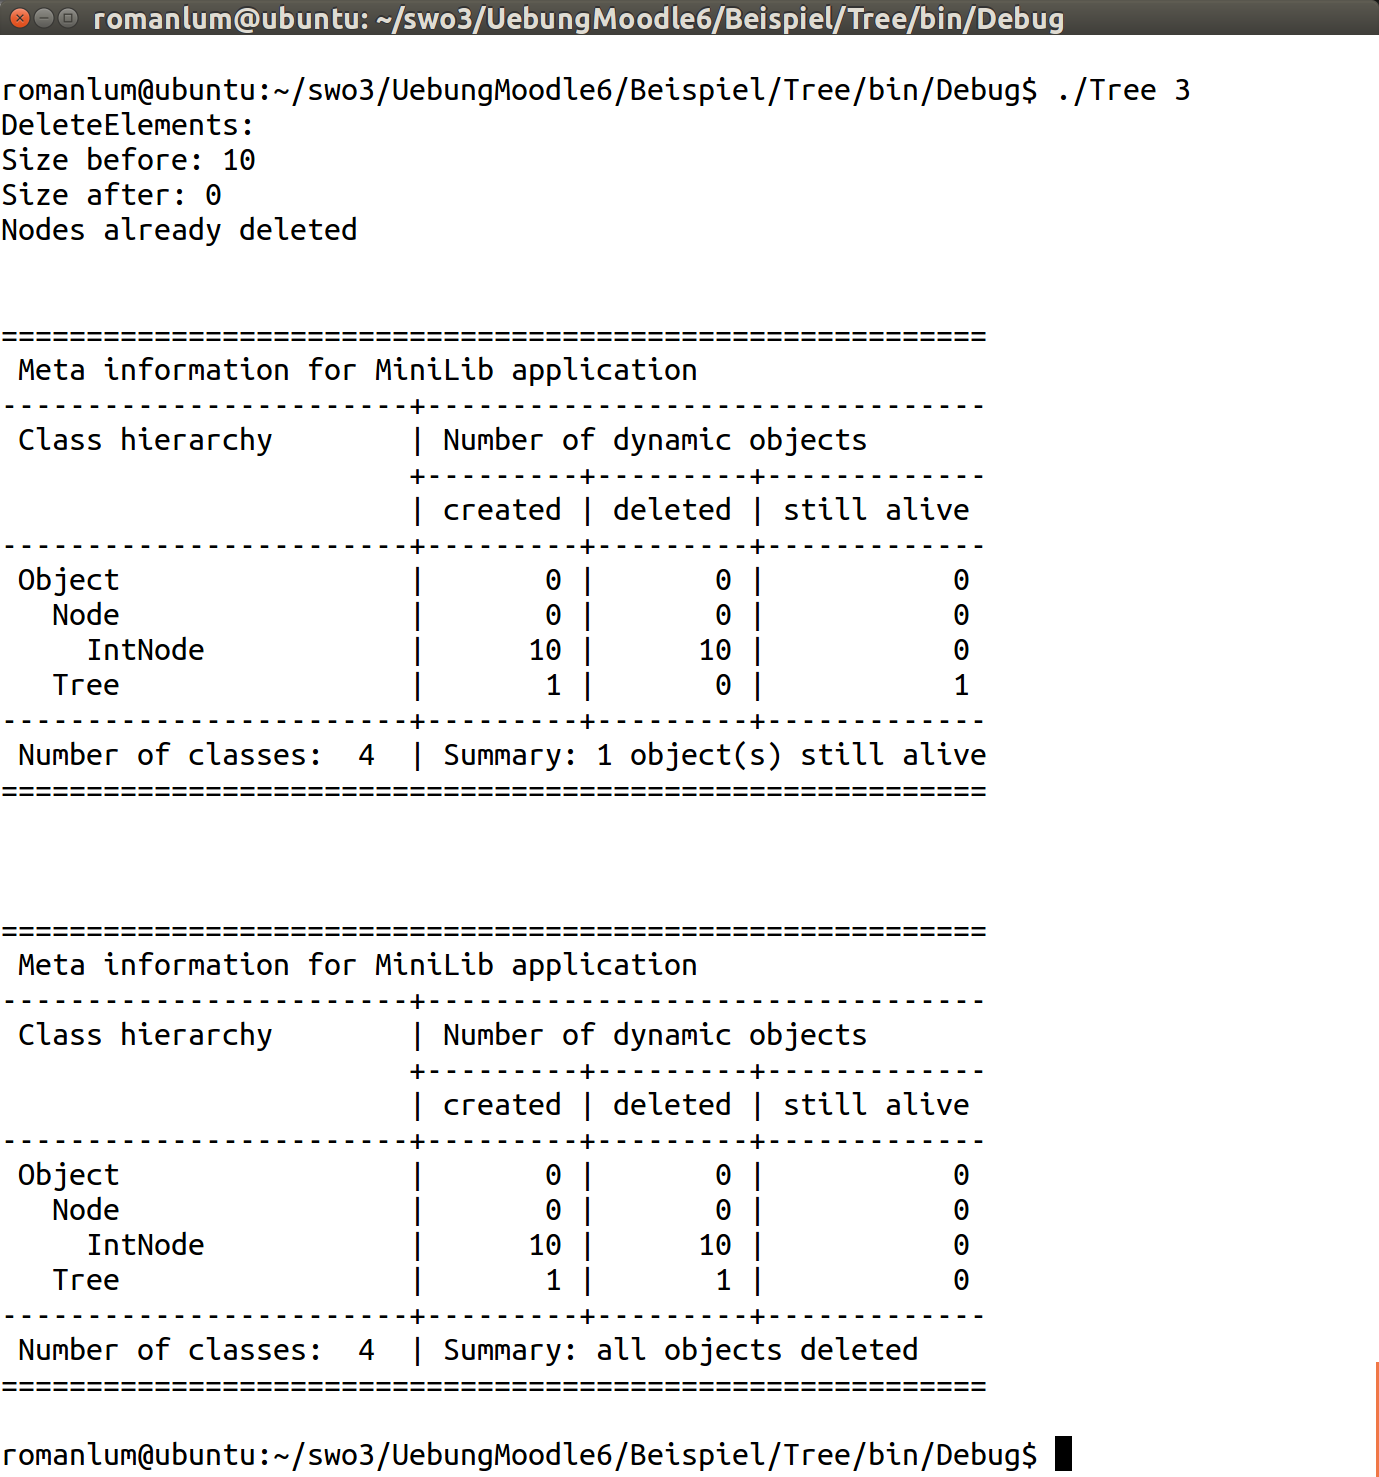
\includegraphics[width=300px]{../Screenshots/3.png}
\end{mdframed}
\begin{mdframed}

\includegraphics[width=300px]{../Screenshots/4.png}
\end{mdframed}
\begin{mdframed}
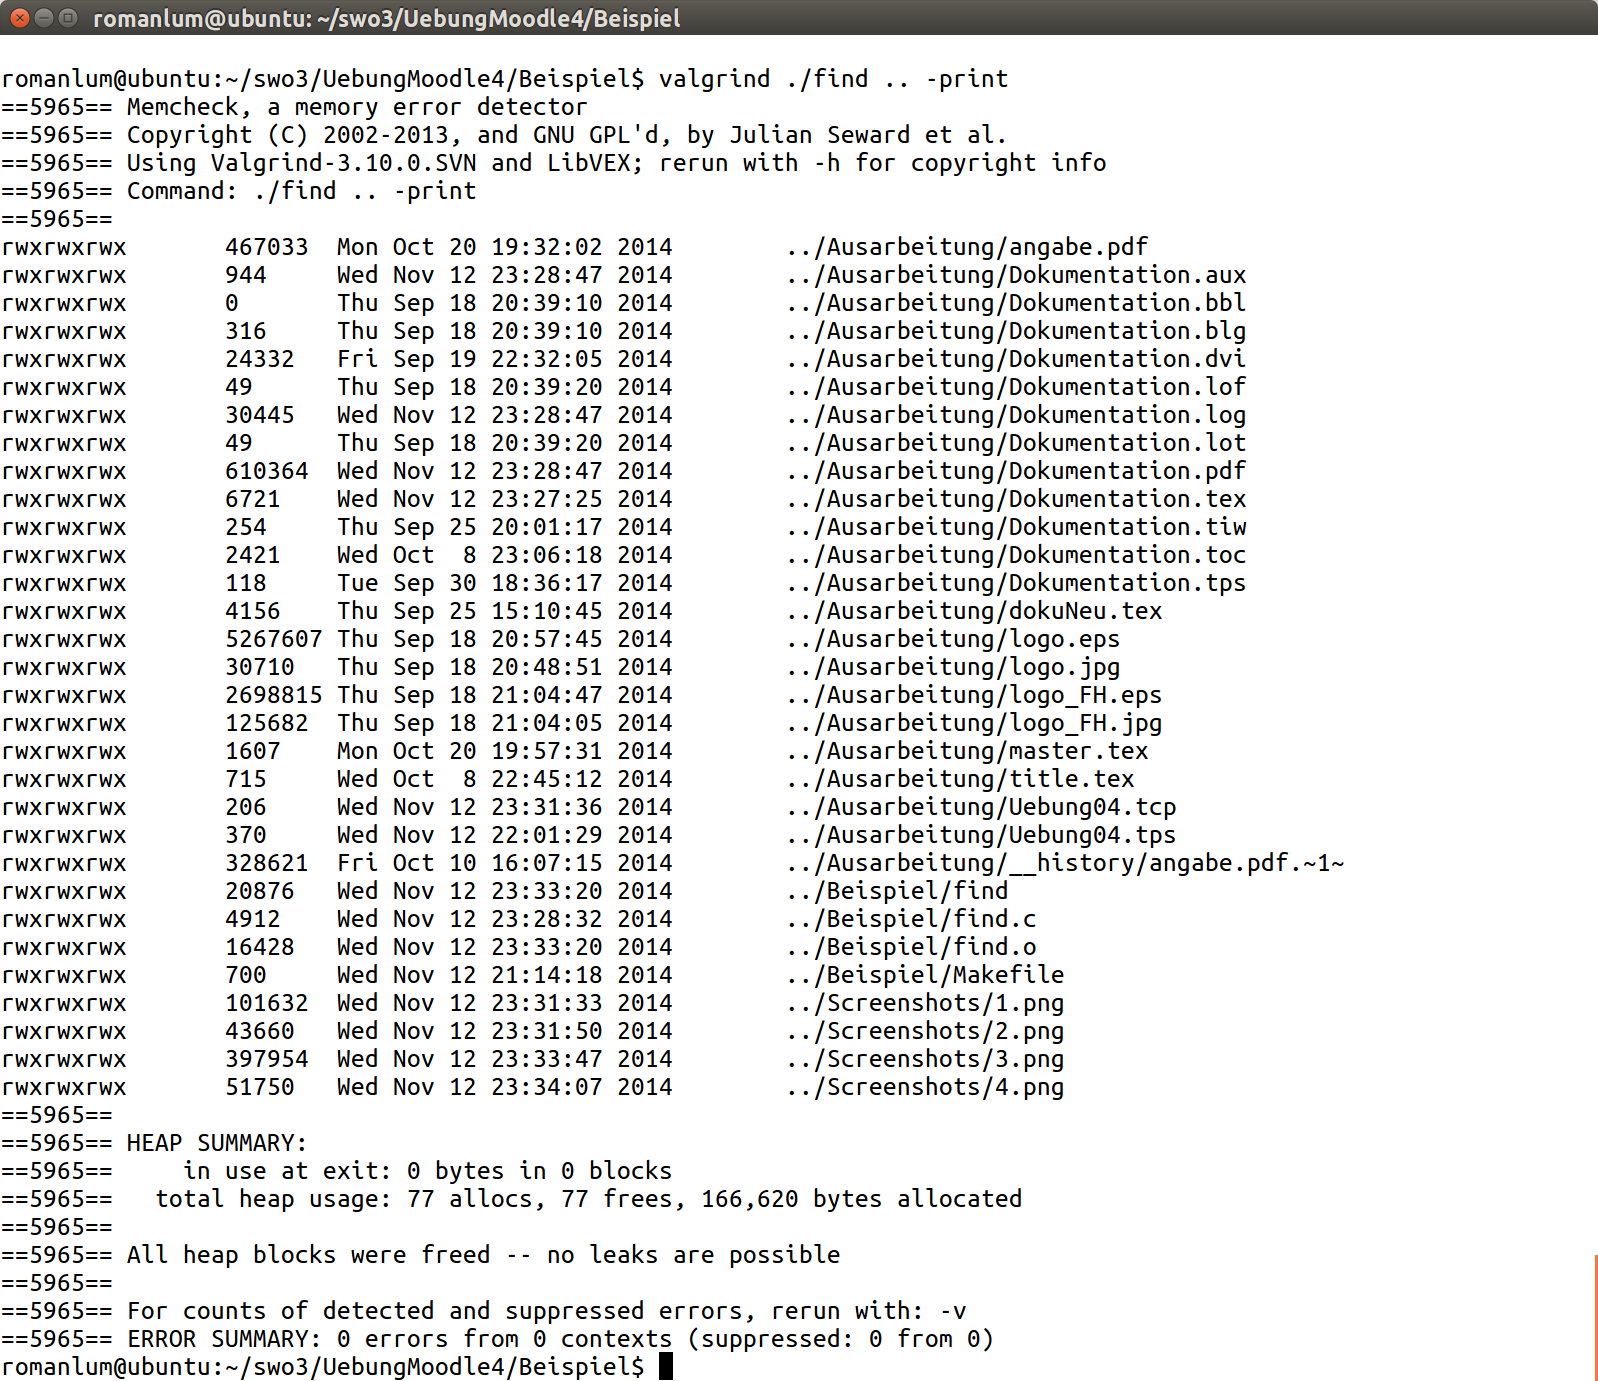
\includegraphics[width=300px]{../Screenshots/5.png}
\end{mdframed}
\begin{mdframed}
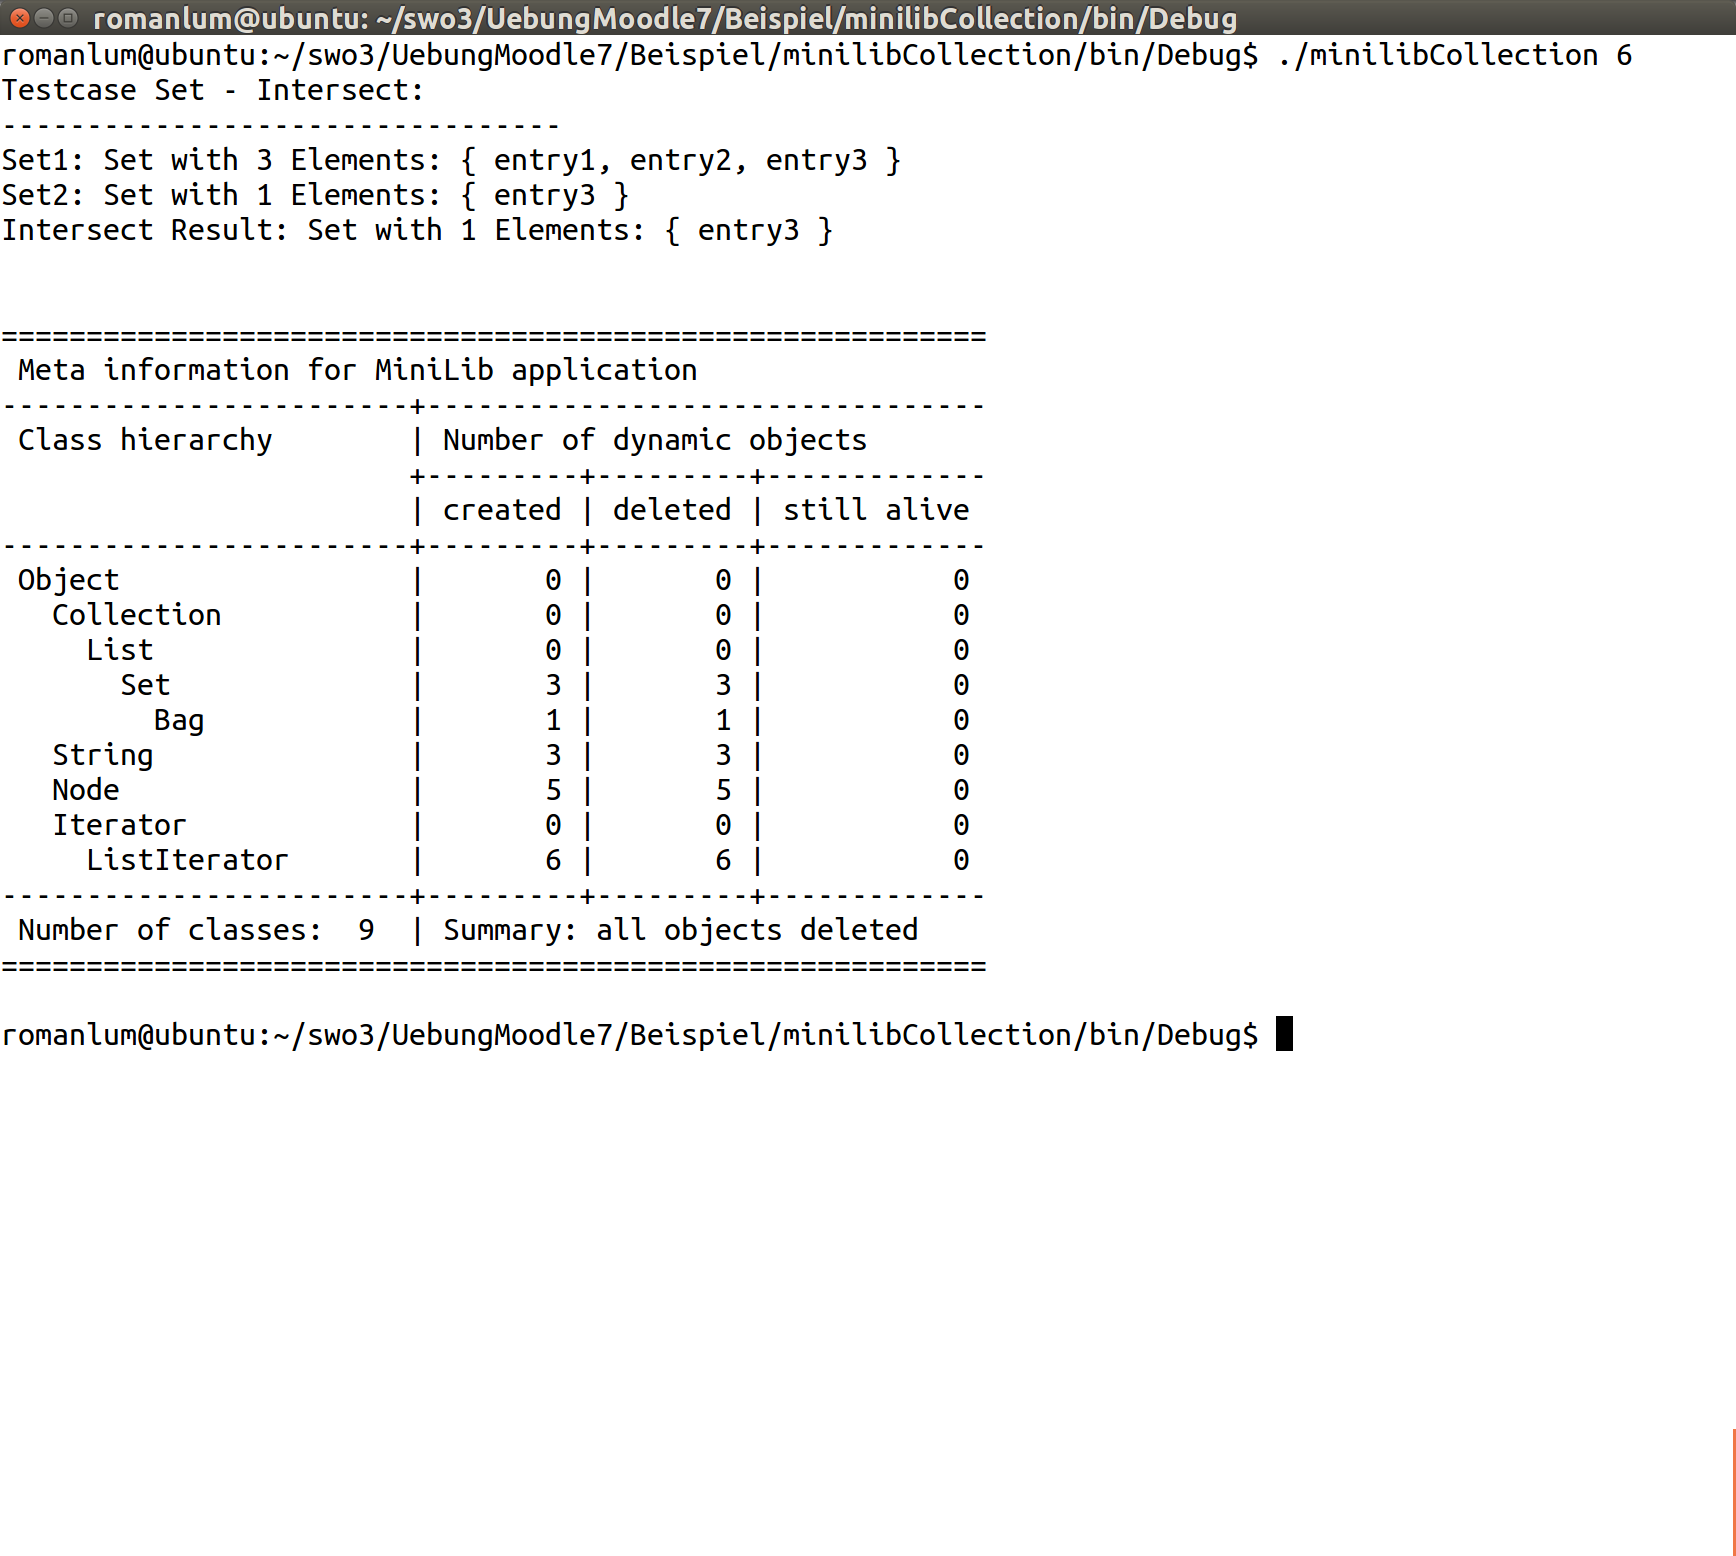
\includegraphics[width=300px]{../Screenshots/6.png}
\end{mdframed}
\begin{mdframed}
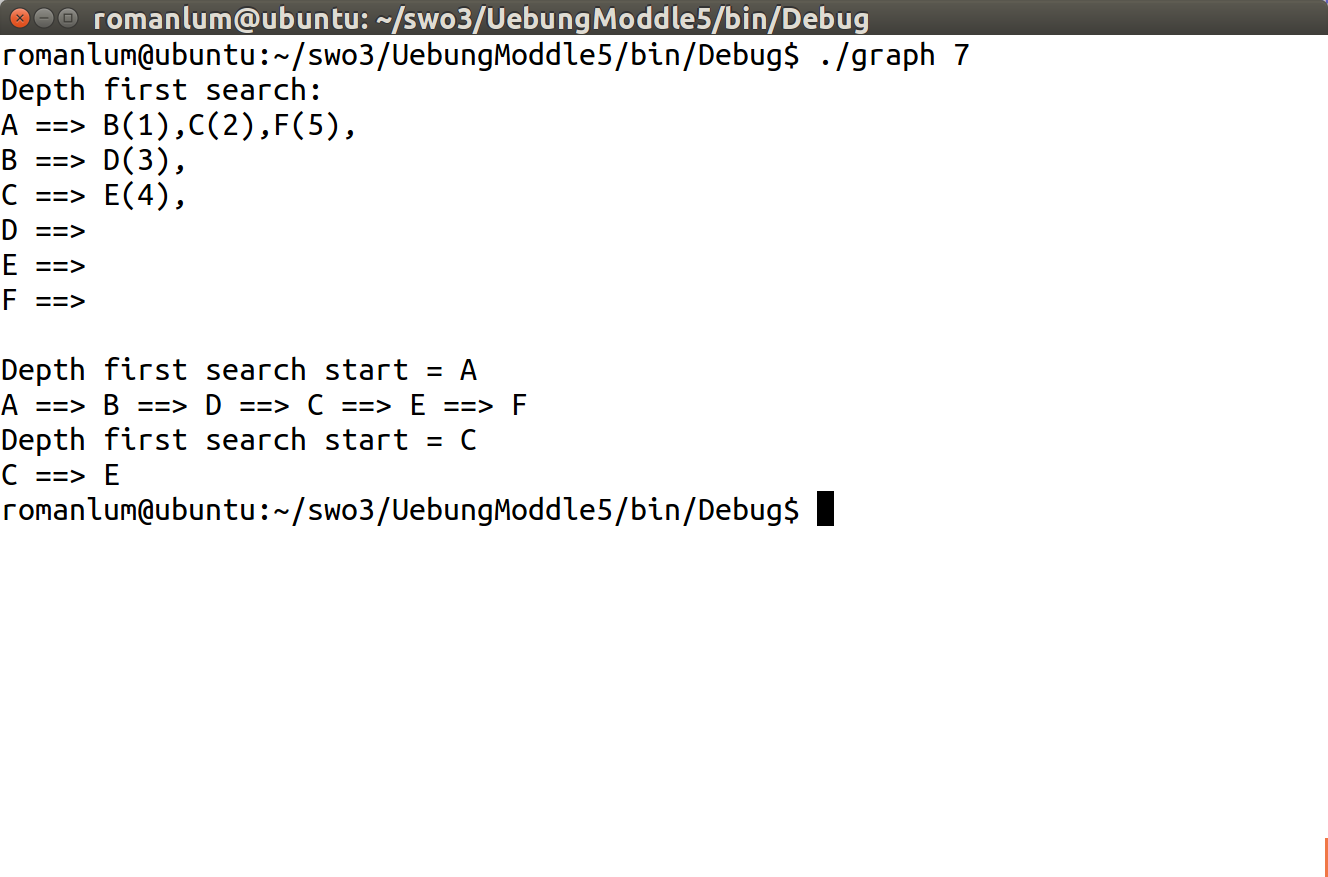
\includegraphics[width=300px]{../Screenshots/7.png}
\end{mdframed}



\end{document}